\section{Experiments}
This section will walk through the experiments conducted in order to answer the question 
of whether the Cross-entropy method or the CMA-ES algorithm can be said to perform better
than the other. The section will provide a discussion on how the experiments are carried out, mainly
in terms of how the Tetris emulator is integrated with Shark and how the game settings were configured.
Furthermore, the section covers an experiment that serves the purpose of indicating whether our implementation
of the Cross-entropy method is similar to the ones in the literature. 
We wish to ensure that both algorithms when competing in learning Tetris, both operate under the 
best performing settings. To satisfy this, a series of experiments with altering settings for each 
algorithm was conducted in the search of the parameter settings to get the best performance from 
each algorithm. Finally, the optimal settings for each algorithm is applied to
the same Tetris game configuration to decide if any significant difference appears.\\
\\
The experiments conducted in this section are all much in the same nature, and the 
results for each experiment is presented mostly in the same fashion. When using some setting 
of the game and the optimizers, the same experiment is executed multiple times, typically 
10 or 30 times. This is because the score of a Tetris controller and the overall 
solution found by the optimization algorithms are influenced by some level of noise.
Due to this noise, the reported performance of an optimization algorithm at a time
is computed as the mean score of it's current solution evaluated 30 times.
\cbcolor{blue}
The experiments will include some configuration of the Tetris emulator which are settings
such as feature set (which in turn translates into dimensionality of the problem),
piece types. Furthermore, the optimization algorithm is chosen and configured according to
the best performing settings determined in the optimization experiments. The
configuration of the optimization algorithm includes setting such as population size
$\populationSize$, parent size $\offspringNumber$ and how many times
to evaluate an agent $\numberOfEvaluations$. The number of evaluations $\numberOfEvaluations$
is how many times each search point/agent from the algorithms are evaluated against the 
Tetris emulator. For every iteration in the algorithm, the current solution is 
evaluated against Tetris emulator 30 times, and the mean of those 30 games are used as
a metric for the current state of learning at the given iteration. When results are presented 
in the following sections, we typically present plots accompanied with tables 
that hold the scores of the algorithms. We have two kinds of plots, one contains all
individual runs with a given configuration and the other shows the mean performance
of all all the runs. The tables will show the mean and quantile scores of the experiments
of a given configuration.\\
\\
In all papers used for reference we haven't seen any experiments with different population
and parent sizes presented side-by-side. All the experiments we've seen
that has applied the Cross-entropy method to Tetris fix the population size to 100. 
However, in our upcoming experiments
CMA-ES and the Cross-entropy method are configured with different population and parent sizes, which means
that we cannot compare the learning curves based on iterations/generations. Instead as described
in section \ref{varifyofce}, using the  
\textit{number of games evaluated} (the number games evaluated, number of agents evaluated and evaluations of the objective function, all refer to the same metric) as comparison reference, equal terms are secured for both algorithms 
in regards to learning speed.
Hence the x-axis represents the total number 
of Tetris games evaluated, 
$\sum_{i = 1}^{\generation} \populationSize \numberOfEvaluations$. 
Meanwhile the y-axis still represents the mean score 
of the centroid agent at iteration $\generation$.\\

\subsection{MDP-Tetris \label{sec:MDPTetris}}

As described earlier, the MDPTetris platform is used for emulating Tetris controllers. 
The source code for the 
platform is freely available at \url{http://mdptetris.gforge.inria.fr/doc/index.html}.
The software implements the simplified version of Tetris as described in 
section \ref{sec:learningTetris} and is written in C. The source code depends on
the GNU Scientific Library\footnote{\url{http://www.gnu.org/software/gsl/}} and
the OpenGL Utility 
Library GLUT/freeGLUT\footnote{\url{http://freeglut.sourceforge.net/}}.
The library implements a set of executable programs. These programs 
allows execution of agents with fixed policies and visualizations
of the Tetris games using OpenGL.\\
\\
The core application of the source code is a function that allows evaluation of 
a controller. This function accepts the configuration of the game one wishes to play,
simulates the game, and returns the number of lines cleared by the agent during the game.
The configuration of the game is mostly done through reading data files that describes 
different qualities of the game. The feature set is read from a file
like the one seen in figure \ref{fig:featfile}. This file defines which features are to be 
considered by the controller by indices. These indices each map to a feature function 
implemented in the MDPTetris source code. The pieces that occur in the game are also read from a file,
which in our case, is just a file that contains the 7 regular pieces from the ordinary game
(see figure \ref{fig:TetrisPieces}). Later in the experiments however, a more difficult version of Tetris
is discussed, which is harder due to more frequent occurrence of pieces which are difficult to place.
To increase the likelihood of these pieces, the piece configuration file was altered to
contain more of the difficult pieces, thus making them occur more often.\\
\\
To perform the actual optimization of the Tetris agents, the Shark library has been applied
with its implementation of CMA-ES and with our own implementation (now a part of Shark
see appendix \ref{app:crossEntropyCode}). The two optimization algorithms in Shark both 
inherits from the abstract class 
\texttt{\lstinline$AbstractSingleObjectiveOptimizer<RealVector>$}. This superclass defines the
abstract interface for an optimizer that can be applied to problems of finding 
solutions of the type \lstinline$RealVector$ that models a real valued vector.
The objective functions in Shark are implemented by writing a class that inherits 
the \lstinline$SingleObjectiveFunction$, which is an interface for an objective function 
that accepts a single real valued vector and returns a real value indicating how well the supplied
vector evaluates against the underlying function. In our source code, we implemented the class names 
\lstinline$MDPTetris$ that inherits the abstract \lstinline$SingleObjectiveFunction$ class.
Thus, our implementation of the objective function offers an abstraction that to Shark, masks
the actual implementation and configuration of Tetris. The effect of this abstraction is that 
no source code from Shark needs to be aware of any details of the actual function, that is Tetris, being optimized.\\
\\
The \lstinline$MDPTetris$ objective function is adjustable in terms of Tetris board size, piece 
configuration file and feature set. When loading the feature set, the dimensionality of 
the function is set to match the number of features which allows the optimizer to 
scale its search space accordingly.
\begin{figure}[h!]
\begin{center}
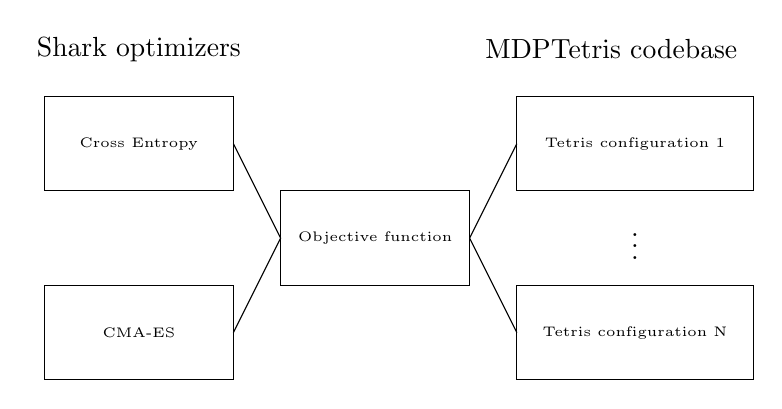
\begin{tikzpicture}[scale=0.6]
\draw  (0,0) rectangle (4,2);
\node at (2,1) {\tiny Objective function};
\draw  (-5,4) rectangle (-1,2);
\node at (-3,3) {\tiny Cross Entropy};
\draw  (-5,0) rectangle (-1,-2);
\node at (-3,-1) {\tiny CMA-ES};
\draw  (5,4) rectangle (10,2);
\draw  (5,0) rectangle (10,-2);
\node at (7.5,1) {$\vdots$};
\node at (7.5,3) {\tiny Tetris configuration 1};
\node at (7.5,-1) {\tiny Tetris configuration N};
\draw (-1,3) -- (0,1) -- (-1,-1);
\draw (5,3) -- (4,1) -- (5,-1);
\node at (-3,5) {Shark optimizers};
\node at (7,5) {MDPTetris codebase};
\end{tikzpicture}
\end{center}
\caption{Fusion of Shark and MDPTetris}
\end{figure}


The source code of the MDPTetris source code 
is accompanied with files that describe the
various existing features, that is files that defines 
the commonly used feature sets. As described, these files contains the identifiers of 
each feature to use, as well as two numbers respectively describing 
the agents reward function and how to evaluate a 'game over' state. 
The number for the reward function has remained unchanged at $0$ 
during all experiments. The "game-over" evaluation, for the
Bertsekas feature set, was initially set to $0$. Setting the 
"game-over" evaluation to $0$ means that the agent will not 
distinguish between regular moves and moves that results in losing
the game. If this setting remains at 0, the agent will always consult the
feature functions to rank its moves, yet setting this value to $-1$
the agent will always, regardless of feature functions, rank moves that ends
the game the lowest.
When running the experiments with this setting as $0$, a large portion
of the agents never exceeded a zero mean score. This occurs presumingly 
due to all agents failing quickly giving the optimization algorithm no 
useful feedback. However, setting the value
to $-1$, meaning that a "game-over" move yields $-\infty$ reward, 
none of the experiments got stuck on only zero scores. An example
of the layout of the feature file can be seen in figure \ref{fig:featfile}.
\begin{figure}[H]
\centering
\begin{lstlisting}
0    <- Describes the reward function
-1   <- Actions leading to game over is avoided at all cost
22   <- The policy contains 22 features
8 0  <- The feature with id 8 initially has weight 0
...  <- The remaining 21 features
\end{lstlisting}
\caption{Example of a file that describes a feature set. \label{fig:featfile}}
\end{figure}

\subsubsection{Game complexity \label{HardTetris}}
Both from other researchers and from the first experiments we executed, 
it quickly became clear that the time consumption of the optimization algorithms cannot be neglected.
Some papers suggests that running 10 executions of the Cross-entropy method
would take more than a month in total. These time estimates 
originates from experiments that were not conducted in parallel,
and on hardware from 2009, yet, the time consumption seemed to 
be a considerable issue.
In order to reduce the runtime of experiments 
to allow us more experiments in the evaluations, 
we can increase the "difficulty" of Tetris, by 
adjusting either the board size and/or adjusting the 
frequency of certain pieces. This has also been described 
before by Amine Boumaza, \citep{boumaza2009}.\\
To increase the difficulty of the game,
in our "Hard" Tetris, the s-block and z-block appear twice as often 
as the other pieces. As described by Boumaza, these pieces are the hardest to
place and will usually cause the player to produce holes and other irregularities
in the game board. Hence, the more frequent these pieces appear, the 
shorter the expected duration of the game.

\begin{figure}[H]
\begin{center}
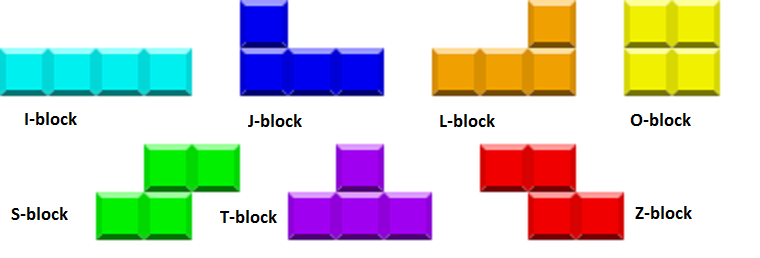
\includegraphics[scale=0.6]{img/Pieces}
\end{center}
\caption{Regular Tetris pieces \label{fig:TetrisPieces}}
\end{figure}

As using the harder version of Tetris, with the hard pieces appearing more frequent, shortens
the expected duration of a game and  the time it takes for an optimization algorithm 
to evaluate a search point, this configuration is indeed useful in searching for optimal parameters
of each algorithm. In the experiments leading to the best configurations of the two 
optimization algorithms, the harder version of Tetris is used. It is mentioned
by Amine Boumaza that using the harder to place pieces more frequently is a good method
for reducing the learning time, however, we have decided to conduct an experiment that explores
how the optimization algorithms behave when the game difficulty is changed.
We do expect that the learning curves develops much the same 
for both the hard and normal game difficulty, however
at lower scores for the harder setting.
To test if the difficulty setting has a significant impact, we used the Bertsekas
feature set (see table \ref{table:bertfeat}) and applied both the Cross-entropy 
Method and CMA-ES on the regular and hard configurations of Tetris.\\

\textbf{Results}\\
Table \ref{table:difficultyRes} renders the results of our experiments 
with with the hard and normal Tetris variants. CMA-ES and the Cross-entropy method 
were each applied 30 times to both game configurations. Table \ref{table:difficultyRes}
shows the means and quantiles of the scores gained in the last iteration.\\
The general settings of the experiments can be seen in the appendix section, \ref{AppendixGameComplexity}.

\begin{table}[H]
\centering
\small
\begin{tabular}{l l r r r r r}
Tetris Type & Optimizer & mean & Q1 & Q2 & Q3\\
\hline
Hard & Cross Entropy & $1633.607$ & $1357.170$ & $1606.565$ & $1938.71$\\
Normal & Cross Entropy & $100059.463$ & $79357.440$ & $105999.500$ & $111047.500$\\
Hard & CMA & $449.352$ & $201.850$ & $300.300$ & $529.350$\\
Normal & CMA & $49760.161$ & $42528.740$ & $49915.700$ & $67764.729$\\
\end{tabular}
\caption{Experiment testing game Normal Tetris against Hard Tetris \label{table:difficultyRes}}
\end{table}

\begin{figure}[H]
\centering
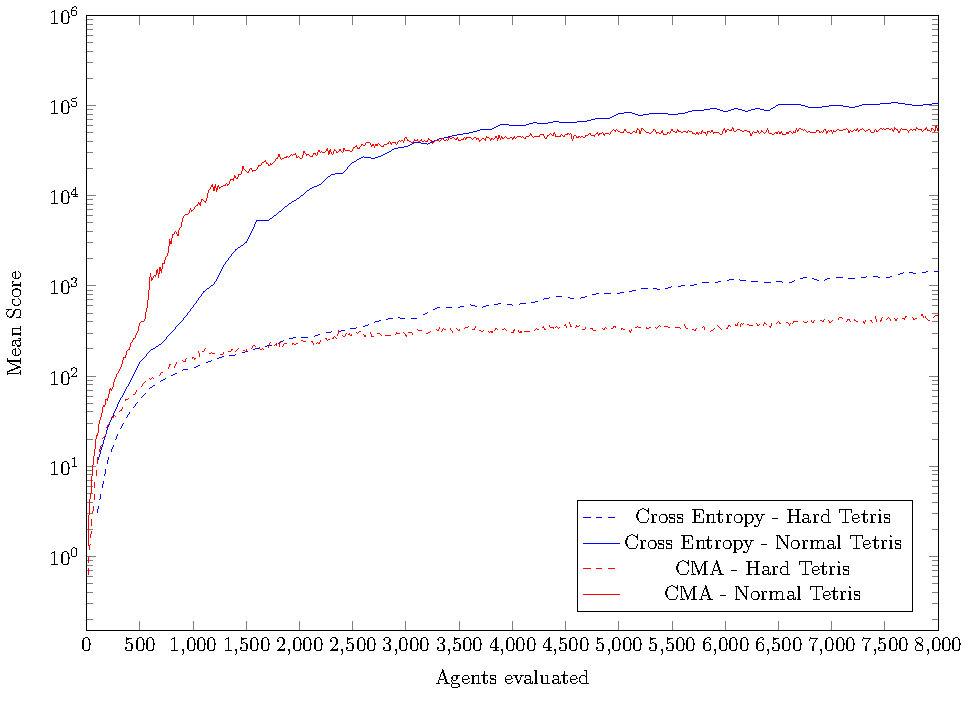
\includegraphics[scale=0.8]{data/complexity/mean/PlotFile.pdf}
\caption{Experiment testing Normal Tetris against Hard Tetris}
\end{figure}

\textbf{Analysis and discussion}\\
The results indicate that using Hard Tetris does not impact 
the general development of the algorithms, meaning we are 
able to use the harder Tetris for further experiments. 
From the graph it appears that the harder Tetris simply 
shifts the score compared to normal Tetris. However, we
will not use Hard Tetris for our final comparison experiments, to ensure that
the final conclusion is based on findings in the domain of the original problem. 
Therefore, we will primarily use Hard Tetris as a faster method for configuring
CMA-ES and the Cross-entropy method, especially when determining the optimal settings.
\\


\subsubsection{Comparison of feature sets  \label{compoffeatureset}}
As described in section \ref{prevWork}, there are different kind of feature sets which
impacts the performance of the agents. In our upcoming experiments, we are going to
use both the Dellacherie and Bertsekas feature set. For our initial comparison experiments
we are going to use the Bertsekas feature set, since other researchers report
a lower score with the Bertsekas feature set compared with the Dellacherie feature set
\citep{scherrer2009}. Compared to the \citep{scherrer2009} experiments, we don't want to maximize the
final score, but rather maximize the score with the lowest possible number of 
games evaluated.\\
It's important to note that we are not going to conduct comparison experiments with different
feature sets in the same experiment, since the algorithms needs to be on equal terms.\\
\\
We want to test whether the feature set has an impact on the performance of the algorithms,
therefore we want to test the two algorithms with both the Dellacherie and Bertsekas feature set.\\
\\
As the results from \ref{HardTetris} suggests, we consider usage of Hard Tetris \citep{boumaza2009} a valid means of asserting the performance difference in the algorithms with altering parameters.
Therefore, to prevent long runtimes, the following games were simulated
using Hard Tetris.\\

\textbf{Results}

In the following figures the mean results of 30 runs of both CMA-ES and the Cross-entropy method is presented. The settings for the Cross-entropy method remains at constant noise
with a noise term of $z^{(\generation)} = 4$ and an initial sigma of $\sigma_0 = 100$, 
and the CMA-ES with $\sigma_0 = 1$.\\
\\
Figure \ref{fig:featuresetCompareBertsekas} shows the experiment with the 
Bertsekas feature set. Which shows that when running the algorithms with a
harder game configuration, the algorithms behave mostly the same as with regular 
Tetris. Namely that CMA-ES converges faster than the Cross-entropy method, 
but is eventually outperformed.

\begin{figure}[H]
\begin{center}
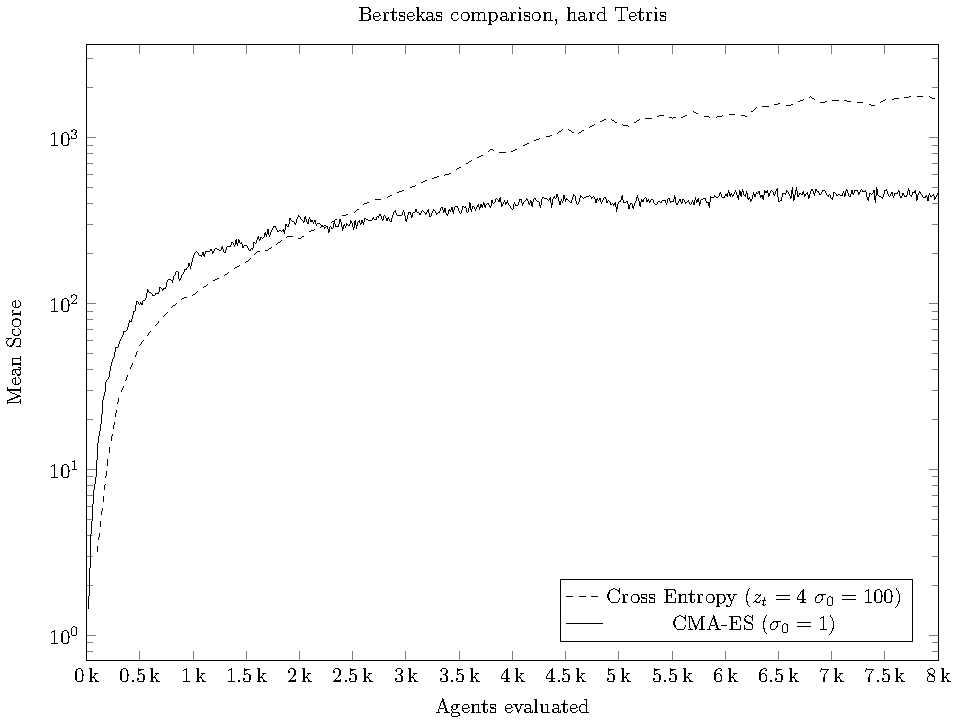
\includegraphics[scale=0.8]{plots/plotBertsekasCmaVsCEHardTetris}
\end{center}
\caption{Comparison between CMA-ES and the Cross-entropy method
using hard Tetris and the Bertsekas feature set 
\label{fig:featuresetCompareBertsekas}}
\end{figure}

When using the Dellacherie feature set a similar behaviour is observed.
However, the convergence seems to occur earlier and with a higher score
(figure \ref{fig:featuresetCompareDellacherie}).

\begin{figure}[H]
\begin{center}
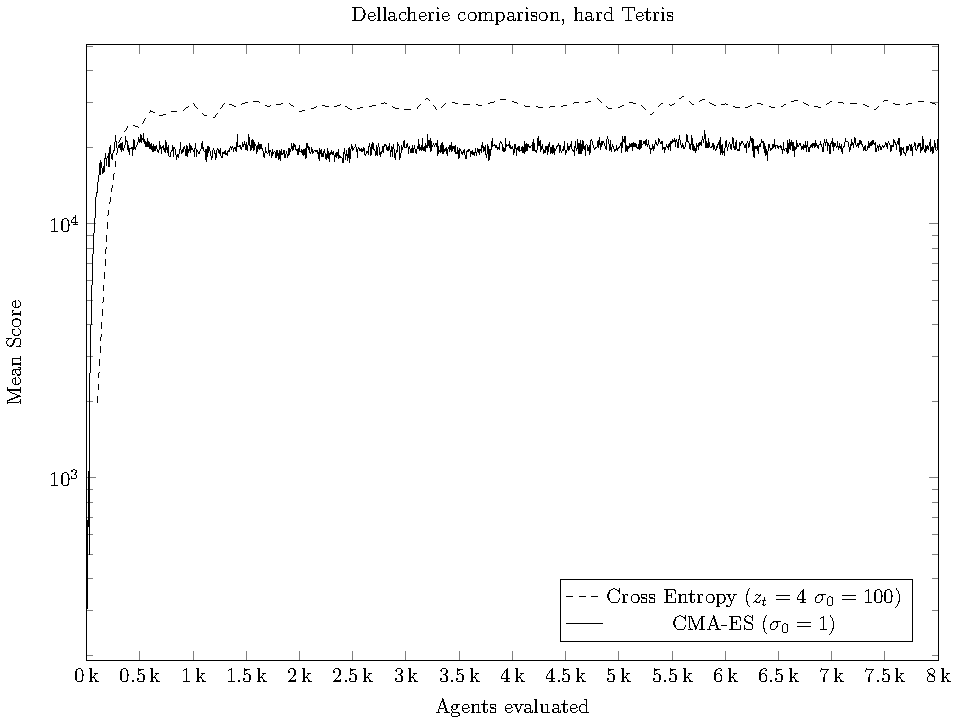
\includegraphics[scale=0.8]{plots/plotDellCmaVsCEHardTetris}
\end{center}
\caption{Comparison between CMA-ES and the Cross-entropy method 
using hard Tetris and the Dellacherie feature set
\label{fig:featuresetCompareDellacherie}}
\end{figure}

\textbf{Analysis and discussion}\\
The experiment with different feature sets indicates that the behaviour 
is not heavily dependant on the feature set.
It appears that changing the feature set simple shifts the score,
but does not affect the development of the graphs.\\
Therefore, we conclude that changing the feature set does not invalidate
the comparison of the two optimization algorithms. This means, that there's
no particular reason for using the Dellacherie feature set instead of the 
Bertsekas feature set, because neither CMA-ES or the Cross-entropy method seems
to benefit differently from the feature sets and the relative performance remains.


\subsection{Setup}

When executing the experiments, various parameters each have 
an impact on the final result of the learning curve. Thus, the parameters
are adjusted, first to match the experiments run by other researchers, 
and later to conduct as fair as possible comparisons between 
the Cross-entropy method and CMA-ES.\\
\\
% agents
The amount of vectors sampled in each generation $\populationSize$
has a high impact on the algorithm performance. By setting $\populationSize$
high, more policies are evaluated per iteration, and leads to a more thorough 
exploration of the search space. Thus the higher $\populationSize$ increases the
chances of finding a better mean for the next iteration.
However, higher $\populationSize$ also results in the
need for more evaluations per iteration. The goal for 
tuning this parameter is then
to set $\populationSize$ high enough to ensure 
exploration of good solutions, and yet 
low enough to avoid unnecessary evaluations.\\
In the implementation of CMA-ES from \shark , 
the algorithm  itself determines
the value of $\populationSize$ according to the 
size of the search space. 
The Cross-entropy method however, does not seem to have a 
general rule for this parameter,
so this value is manually adjusted to fit the 
problem as well as possible.\\
\\
% offspring
As both of the optimizing algorithm uses a subset of the sampled vectors
from a generation to update the distribution parameters, the number of 
offspring $\offspringNumber$ influences how the next generation is sampled.
By setting the value too high, the algorithm risks ceasing to progress any 
further since the updated mean would be too close to the previous one to 
significantly make a difference. By setting the value too low,
the risk of reaching a local optimum increases since the high-scoring agents
might have reached their high performance by chance.\\
The CMA-ES itself manages setting $\offspringNumber$ and the Cross-entropy method
is set according to the problem. Most authors that uses the Cross-entropy method for Tetris
sets the offspring size to $10\%$ of population size, that is 
$\offspringNumber = \lfloor 0.1 \cdot \populationSize \rfloor $.\\
\\
% Number of games per iteration
The number of games, $\numberOfEvaluations$, 
is the number of games  which each agent 
plays in each iteration. An agent's score is defined as the 
mean of the score of these 
$\numberOfEvaluations$ games.
We want this value low as possible, because as with the number of
agents, $\populationSize$, The number of games, $\numberOfEvaluations$, 
is another major factor in the run-time of the algorithm.
As Tetris is stochastic by nature, the score deviates a lot, 
even when the
same agent with the same policy plays multiple games. 
Hence, when assessing the true
performance of a policy it's rarely enough to play just few games. Thus, setting 
$\numberOfEvaluations$ high increases the likelihood of correctly choosing the best 
agents, yet, it also causes longer run times of the experiments.\\
\\
% Noise factor
Specific to the Cross-entropy method, 
most authors report that the performance of the 
algorithm increases dramatically when the sampling 
distribution is associated with
a noise term. The different types of 
noise are described in section \ref{CrossEntropy}.
The noise term is adjusted in order to 
prevent the algorithm from reaching a local optimum.
The current research shows that noise terms of $\noise^{(\generation)} = 4$ and 
$\noise^{(\generation)} = max \left( 5 - \generation / 10 \right)$ 
\citep{thiery:09} produces the best results.
The constant noise (such as $\noise^{(\generation)} = 4$) ensures that the algorithm
never settles in a too small area from which it samples, and forces it to explore
solutions that are further away from the mean. The further the 
algorithm progresses, 
the less noise is assumed needed, as the mean should approach a global optimum. to
address this, the linear decreasing noise 
is applied as it will lower the noise term
as the algorithm progresses.\\
\\
For the various experiments, these 
parameters will be tuned for the specific purpose 
at hand. In the verification of the Cross-entropy method, the parameters are set 
to match those reported in similar papers (\cite{thiery:09}, \cite{szita:06}).
In the comparison of the two algorithms, the parameters will be set such that 
the Cross-entropy method operates under as 
similar conditions as CMA-ES, to ensure an unbiased 
comparison.







\subsection{Verification of our implemented of the Cross-entropy method \label{varifyofce}}

Because the \shark\ library already contains an implementation of 
CMA-ES, but not an implementation of the Cross-entropy method, we extended the library
with our own implementation of the algorithm.\\
In order to verify the correctness of the implementation, 
we used the same experiments as used by 
Christophe Thiery and Bruno Scherrer \citep{thiery:09}. 
These experiments were used by Thiery and Scherrer to 
verify their own Cross-entropy method implementation with various types of noise correction. 
Therefore, we will perform the same experiments to verify our 
own contribution to the \shark\  library, by trying to achieve the same results.\\
\\
The setup is mirrored from the paper \citep{thiery:09}, 
with 100 agents ($\populationSize = 100$) per iteration,
and using the $\offspringNumber = 10$ best vectors
for the update step. After each iteration, 
an agent with the updated mean 
plays 30 games and the mean of these scores are recorded for the
learning curve.\\
During evaluation each agent plays one game, that is $\numberOfEvaluations = 1$.
A minor derivation from the figures present in \citep{thiery:09}, is 
the unit along the x-axis in the learning curve plots indicates 
the iteration number. As the experiments in this two algorithms
width variable population sizes are compared, the x-axis in all plots
indicated the number of Tetris games played during the learning. In one 
generation $\populationSize$ agents each play $\numberOfEvaluations$ games and hence
advance the x-axis by $\populationSize \numberOfEvaluations$.\\

\begin{figure}[H]
\begin{center}
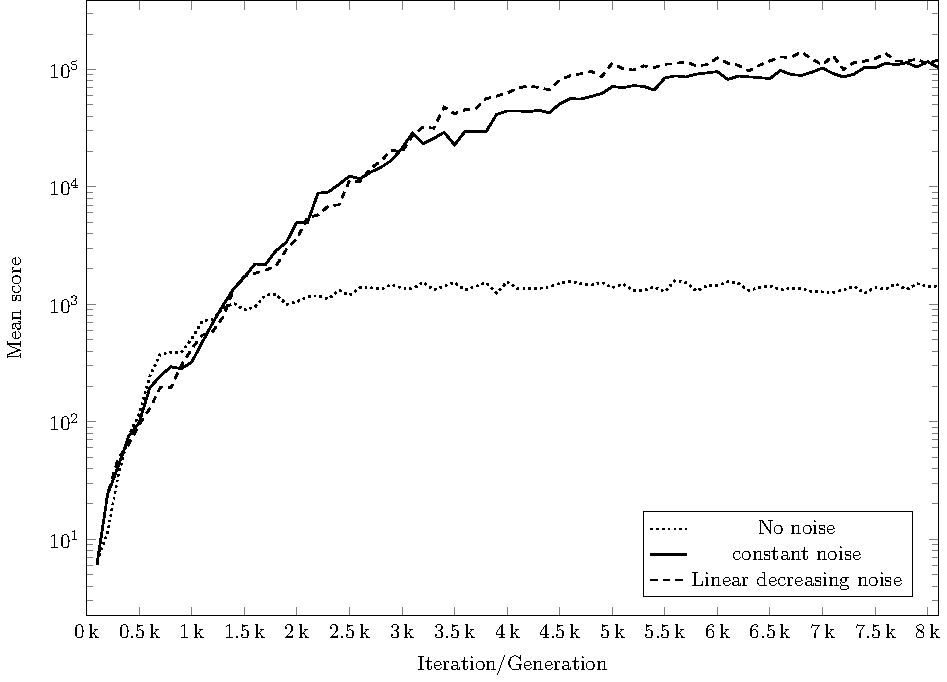
\includegraphics[scale=0.8]{plots/meansPlot}
\end{center}
\caption{Cross-Entropy mean performance \label{fig:cemean}}
\end{figure}

\clearpage
\begin{figure}[H]
\begin{center}
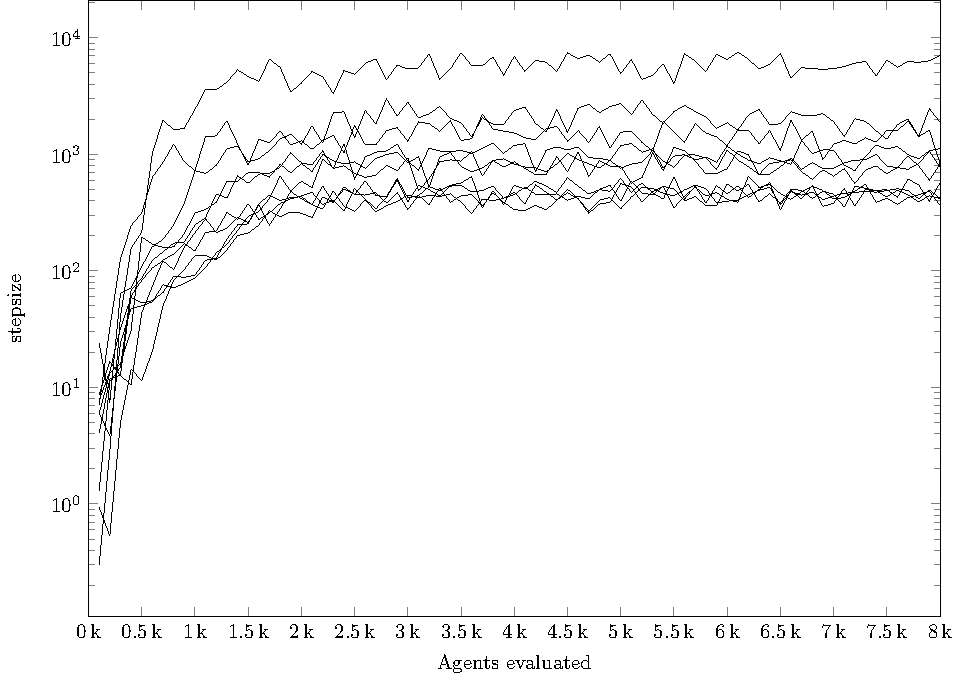
\includegraphics[scale=0.48]{plots/noNoisePlot}
\end{center}
\caption{No noise \label{fig:ceNoNoise}}
\end{figure}
\begin{figure}[H]
\begin{center}
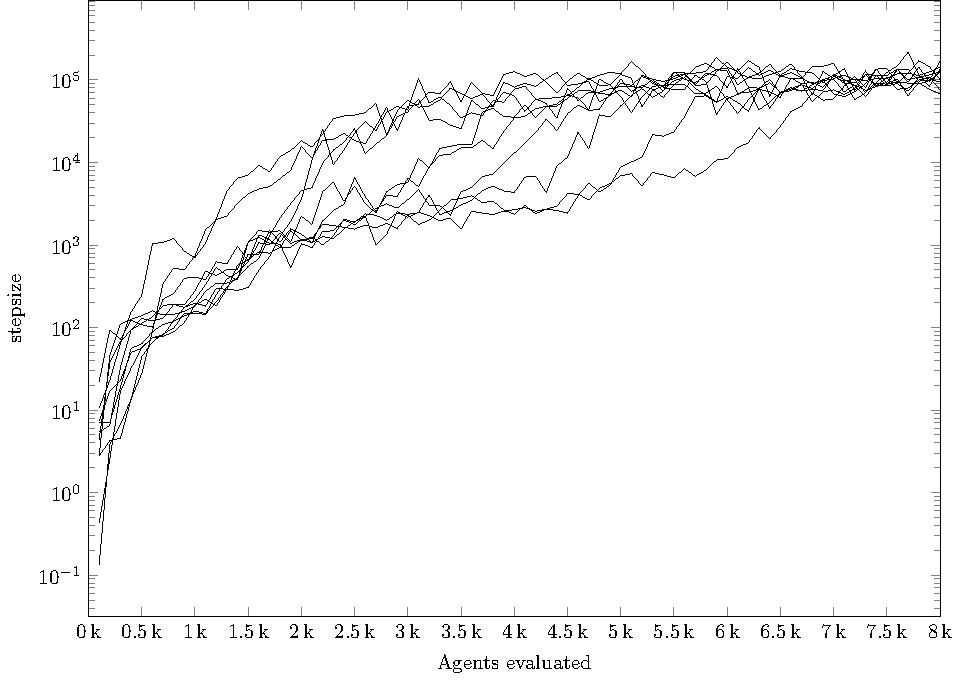
\includegraphics[scale=0.48]{plots/constantNoisePlot}
\end{center}
\caption{Constant noise \label{fig:ceCnstantNoise}}
\end{figure}
\begin{figure}[H]
\begin{center}
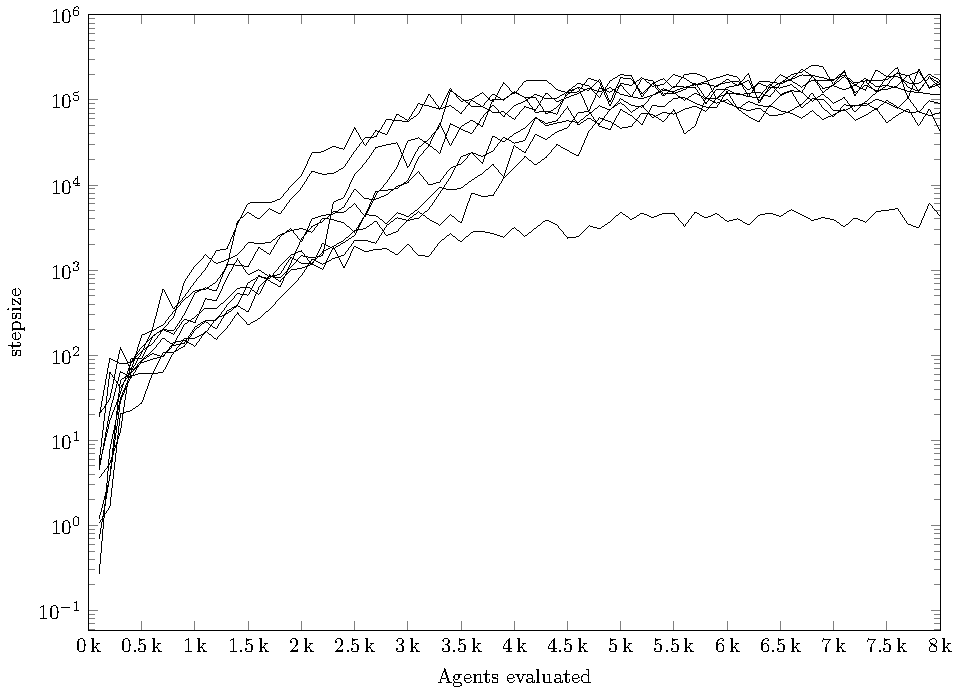
\includegraphics[scale=0.48]{plots/linearNoisePlot}
\end{center}
\caption{Linear decreasing noise \label{fig:ceLinNoise}}
\end{figure}

Figure \ref{fig:ceNoNoise}, \ref{fig:ceCnstantNoise} and
\ref{fig:ceLinNoise} shows 10 runs of each noise type. Figure
\ref{fig:cemean} shows the mean graph for each of the noise types.
The goal of these experiments were to replicate the experiments 
reported in \citep{thiery:09}. As the results seen from our experiments
to a high degree resemble those reported by Thiery et. al, we conclude
that our Cross-entropy method implementation works similar to theirs.\\
\\
When evaluating the score of the agent we also want to compute the confidence
interval in verifying the implementation of the Cross-entropy method. The mean agent plays 30 games
which leads to a confidence interval of $\pm36\%$ around the estimated mean,
which is similar to the confidence intervals in \citep{scherrer2009}.\\
By looking at the individual graphs for the different noise types 
(Figure \ref{fig:ceNoNoise}, \ref{fig:ceCnstantNoise} and
\ref{fig:ceLinNoise}), we get the following average scores.\\
\\
\textbf{Without noise (figure \ref{fig:ceNoNoise})}: The learning curve
stabilizes after 1,500 agents evaluated. And as it can be observed the
score variates much for the different executions between a score of 300 and 6,000
rows. This results in an average score of 1,400$\pm36\%$ rows.\\
\textbf{Constant noise (figure \ref{fig:ceCnstantNoise})}: 
The 10 executions reaches equivalent performances at some point, 
with a score between
54,000 and 154,000. This results in an average score of 105,000$\pm36\%$ rows.\\
\textbf{Linear decreasing noise (figure \ref{fig:ceLinNoise})}:
Most of the executions of this noise type settles around 200,000.
However, a single execution settled at a score of only around 5,000.
The mean performance of this noise type yielded a score of
120,000$\pm36\%$ \\

Based on the mean graphs and confidence interval compared to other papers, we can
hereby verify that our implementation of the Cross-entropy method works as intended. Even though the
experiments with linear decreasing noise in this case seems to outperform
the constant noise, other runs with linear decreasing noise ended in a mean 
performance of only 90,000$\pm36\%$. Yet, the constant noise is both from our
own experiments, and described in other research, noted to be the most reliable
noise type for reaching high scoring controllers \citep{scherrer2009}. 
Due to this, the constant noise is used in the 
benchmarking against CMA-ES.\\





\subsection{Optimal settings 
for the Cross-entropy method \label{optimalsettingsce}}

In this section we will determine the optimal settings for \begin{changebar}
\cbcolor{blue}
the Cross-entropy method
\end{changebar} through testing
of various adjustable parameters.\\
Compared to CMA-ES, the Cross-entropy method has fewer customizable parameters, more specifically 
only population-parent size and games played per agent.

\subsubsection{Population and selection size}
Other researchers run the Cross-entropy method with population size of
$\populationSize = 100$ and an offspring corresponding to 10\% of 
the population size, resulting in $\offspringNumber = 10$. As it's not 
discussed why this exact setting is applied, various settings of the Cross-entropy method
was executed to asses the performance of other configurations
in our experiments.
The experiments includes different population sizes 
$\populationSize \in \{12, 22, 50, 100, 200\}$ and offspring 
sizes of either $10\%$ and $50\%$ (since the CMA-ES algorithm by default
uses $50 \%$ selected vectors). 
A summary of the experiments can be seen in figure \ref{CEConfigTest}
on page \pageref{CEConfigTest}.

\begin{figure}[H]
\centering
\begin{tabular}{r r | r r r r}
$\populationSize$ & $\offspringNumber$ & mean & Q1 & Q2 & Q3\\
\hline
13 & $10\%$  & 1585,3     & 93,0      & 113,5        & 220,7\\
13 & $25\%$  & 30.496,9   & 15.222,1  & 20.264,2     & 39.019,8\\
13 & $50\%$  & 39.824,2   & 26.457,0  & 33.663,4     & 49.743,7\\
22 & $10\%$  & 35.841,6   & 20.391,9  & 42.045,5     & 48.464,6\\
22 & $25\%$  & 80.884,9   & 56.042,5  & 71.900,2     & 78.653,4\\
22 & $50\%$  & 52.887,4   & 23.531,9  & 42.161,0     & 83.144,1\\
50 & $10\%$  & 95,623,1   & 82.738,9  & 93.388,9     & 111.351,5\\
50 & $25\%$  & 110.525,0  & 103.128,1 & 111.195,5    & 121.974,4\\
50 & $50\%$  & 69.130,7   & 52.511,0  & 64.351,6     & 91.488,6\\
\hdashline
100 & $10\%$ & 115.868,7  & 84.368,5  & 122.238,5    & 146.457,0\\
\hdashline
100 & $25\%$ & 70.011,1   & 58.008,0  & 69.588,2     & 80.432,7\\
100 & $50\%$ & 22.910,4   & 4.037,7   & 14.353,7     & 47.215,9\\
200 & $10\%$ & 85.181,7   & 45.201,5  & 96.803,1     & 117.578,0\\
200 & $25\%$ & 32.894,6   & 8688,7    & 25.333,1     & 58.434,8\\
200 & $50\%$ & 946,4      & 585,0     & 802,5        & 1.267,7
\end{tabular}
\caption{the Cross-entropy method configuration test, 
see Appendix \ref{appendixCrossEntropyConfig} for the full plots 
of the experiments.  \label{CEConfigTest}}
\end{figure}

The experiments with different population and parent sizes
does not seem to support a choice for any other configuration 
than the mostly commonly used 
$\populationSize = 100$ and $\offspringNumber = 10$. \\
However, with a configuration of $\populationSize = 50$ and $\offspringNumber = 12$ convergence
is achieved faster (see figure \ref{fig:bestConfCE}). This means that the score limit is reached faster, which
results in longer computation time, than the $\populationSize = 100$ and $\offspringNumber = 10$
configuration. In other words, the $\populationSize = 100$ and $\offspringNumber = 10$ configuration 
is therefore preferred since it takes shorter computation time and the end-result is similar compared
to the $\populationSize = 50$ and $\offspringNumber = 12$ configuration, even though the latter 
configuration from our expriments converged faster. The experiments also apppears
to suffer from a high noise, yet both the mean and the quantiles favor the 
extensively tested the Cross-entropy method configuration of $\populationSize = 100$ and $\offspringNumber = 10$.

\begin{changebar}
\cbcolor{blue}
\begin{figure}[H]
\begin{tabular}{@{}l@{}l@{}}
\includegraphics[scale=1]{plots/ce_ConstantNoise_l50_o12_all} &
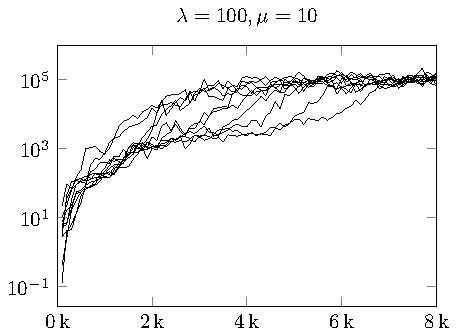
\includegraphics[scale=1]{plots/ce_ConstantNoise_l100_o10_all}
\end{tabular}
\caption{The two best configurations of the Cross-entropy method 
\label{fig:bestConfCE}}
\end{figure}
\end{changebar}

\subsubsection{Games per agent \label{GamesPerAgentCESection}}
Another parameter we can adjust is the number of 
games played each agent plays per generation. By playing
multiple games with each agent and using their 
mean score to compute the next generation mean. This
secures a higher chance of a better offspring generation,
but at the cost of more games
evaluated.\\
Table \ref{GamesPerAgentCE} shows the different values of
games per agent we are going to be
testing.

\begin{table}[H]
\centering
\begin{tabular}{c c c}
Population Size & Parent size & Games per Agent\\
\hline
$13$ & $10\%$ & 1/3/5/7/10\\
$13$ & $25\%$ & 1/3/5/7/10\\
$13$ & $50\%$ & 1/3/5/7/10\\
$22$ & $10\%$ & 1/3/5/7/10\\
$22$ & $25\%$ & 1/3/5/7/10\\
$22$ & $50\%$ & 1/3/5/7/10\\
$50$ & $10\%$ & 1/3/5/7/10\\
$50$ & $25\%$ & 1/3/5/7/10\\
$50$ & $50\%$ & 1/3/5/7/10\\
$100$ & $10\%$  & 1/3/5/7/10\\
$100$ & $25\%$  & 1/3/5/7/10\\
$100$ & $50\%$ & 1/3/5/7/10\\
$200$ & $10\%$ & 1/3/5/7/10\\
$200$ & $25\%$ & 1/3/5/7/10\\
$200$ & $50\%$ & 1/3/5/7/10
\end{tabular}
\caption{Games per agent of the Cross-entropy method experiment setup\label{GamesPerAgentCE}}
\end{table}

The experiments includes different games per agent of $\{1,3,5,7,10\}$. By increasing the number of games 
played per agent, we are increasing the evaluation cost by a multiplication factor in exchange for a more 
accurate evaluation of each agent. This is to avoid misconceiving poor performing agents
for good ones, as multiple evaluations will decrease the chance the agent having 
'lucky games'. However, we wish to find 
the best performing configuration with the lowest cost and maximum benefit, and evaluating multiple 
times will increase the function cost.\\
\\
\textbf{Results}\\
The total number of configuration experiments is 75, with 30 individual experiments each,
resulting in a total of
\begin{changebar} 
2,250
\end{changebar} 
individual experiment runs. These results are all included in 
appendix \ref{appendixCEPopulationParent}.\\
Below in table \ref{CEBestConfigTable} and figure \ref{CEBestConfigPlot}, the five best
best resulting configurations are depicted. We chose these by first selecting the best 
configuration of each Population-Parent size. This resulted in three
configurations for each Population-Parent size, which we then compared to determine the best
configuration for each Population-Parent size. Which is depicted in table \ref{CEBestConfigTable} and figure \ref{CEBestConfigPlot}.
\begin{table}[H]
\centering
\small
\begin{tabular}{r r r r r r r}
Population & Parent & Games per Agent & mean & Q1 & Q2 & Q3\\
\hline
$12$ & $6$ & 10 & $2109.837$ & $1802.968$ & $2021.165$ & $2276.652$\\
$22$ & $5$ & 5 & $2371.793$ & $2013.168$ & $2412.815$ & $2708.931$\\
$50$ & $12$ & 5 & $2749.991$ & $2605.171$ & $2702.400$ & $2835.960$\\
$100$ & $25$ & 3 & $2776.560$ & $2397.691$ & $2742.950$ & $3027.541$\\
$200$ & $50$ & 1 & $2950.767$ & $2564.118$ & $2841.065$ & $3377.189$\\
\end{tabular}
\caption{Best configurations of all population sizes - the Cross-entropy method \label{CEBestConfigTable}}
\end{table}

\begin{figure}[H]
\centering
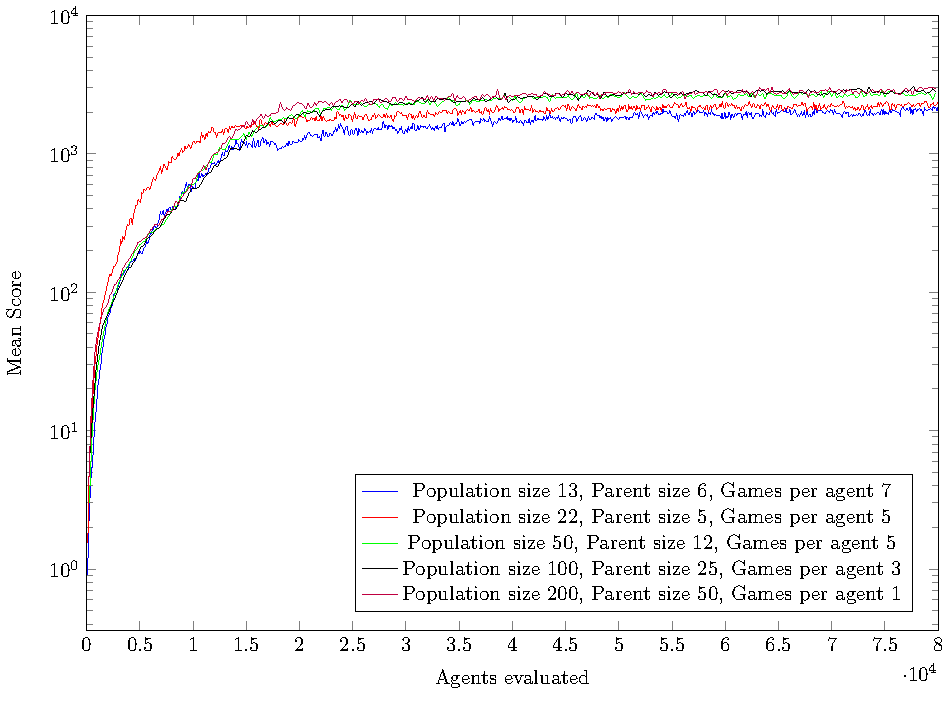
\includegraphics[scale=0.8]{data/ce_population_offspring/bestofall_population/PlotFile.pdf}
\caption{Best configurations of all population sizes - the Cross-entropy method \label{CEBestConfigPlot}}
\end{figure}

From table \ref{CEBestConfigTable} and figure \ref{CEBestConfigPlot}, we can see that population size 50 with parent size 12 and 5 games per agent, population size 100 with parent size 25 and 3 games per agent, and, population size 200 with parent size 50 and 1 game per agent, performs almost identically.\\

\textbf{Discussion and analysis}\\
From the graph and the table depicting the quantiles, it appears that the configuration
population size 200 with parent size 50 and 1 game per agent yields the best performance. 
It achieves the highest score with the fastest convergence of all the candidate solutions
we have listed.\\
Therefore, we will be using this configuration for the tuned comparison experiments.


\subsection{Optimal settings 
for CMA \label{optimalsettingscma}}

When finding the optimal settings for CMA we have a larger set of parameters we can adjust compared
to Cross Entropy. Again, as the same with Cross Entropy, we can adjust the population/parent size and
games per agent. Furthermore we can adjust the initial step-size, lower bound and recombination type.\\
The following sections will go into detail how these parameters affect the performance of CMA
algorithm. In the last section we will perform experiments to determine the optimal settings.

%In previous sections we focused on tuning Cross Entropy for the Tetris 
%problem. Whereas we deliberately chose not to tune CMA due to its implementation 
%into the Shark library \citep{shark08}. However, experiments with the "out of 
%the box" CMA from Shark, with default settings vs the tuned Cross Entropy
%resulted in CMA reaching convergence very fast but not achieving the same point
%limit as Cross Entropy.\\

\subsubsection{Recombination type}
Furthermore, CMA also has a unique formula for calculating the updated mean,
called the 'Recombination type' \ref{CMAtheory}. Where the recombination type
determines how much influence each of the offspring vectors has on the next
generation. Built into the CMA algorithm is three methods of recombination. 
\begin{itemize}
\item EQUAL, Each of the offspring vectors has equal influence in the generated mean.
\item LINEAR, The best of the offspring vectors has more influence. 
\item SUPERLINEAR, The vectors are weighted with a logarithmic equation.
\end{itemize}
\begin{changebar}
As default, CMA uses Super Linear recombination. However, Tetris is a problem
with multiple local optimums and heavy noise in its search space. 
\end{changebar}
This means, though a vector may be the best in its generation,
it could be a nearby local optimum. Therefore,
Super Linear recombination may not be the optimal recombination type for the Tetris problem.\\

The recombination types are covered in section \ref{CMAtheory} on 
page \pageref{eq:recomType}.


\subsubsection{Population and selection size}
By adjusting the population size to that similar of Cross Entropy, we are able
to get a fair comparison between the two algorithms, given each generation will
contain the same number of agents. By setting the population and parent size
to the same values, we in effect test if the covariance matrix and the step-size
control has a impact on the algorithm performance compared to Cross Entropy
which does not have the features.\\
Table \ref{CMAPopulationSelectionConfigTest} displays the values that we are going
to test for the population and selection size.

\begin{changebar}
\cbcolor{blue}
\begin{table}[h]
\centering
\begin{tabular}{r r}
Population size, $\populationSize$ & Parent size, $\offspringNumber$\\
\hline
$12$ & $1$\\
$12$ & $3$\\
$12$ & $6$\\
$22$ & $2$\\
$22$ & $5$\\
$22$ & $11$\\
$50$ & $5$\\
$50$ & $12$\\
$50$ & $25$\\
$100$ & $10$\\
$100$ & $25$\\
$100$ & $50$
\end{tabular}
\caption{CMA-ES configuration for population and parent size \label{CMAPopulationSelectionConfigTest}}
\end{table}
\end{changebar}

The experiments includes different population $N \in \{12,22,50,100\}$ and offspring sizes of either
10\%, 25\% and 50\%. We use 10\% because of the Cross Entropy recommended selection size, while
we use 25\% because of CMA-ES's standard selection size for the EQUAL recombination type. 
Furthermore we use 50\% because of CMA-ES's standard selection size for the LINEAR and SUPERLINEAR 
recombination type.

\subsubsection{Games per agent \label{CMAGamesPerAgentSection}}
As with Cross Entropy we can also adjust the number of games each agent plays per generation.
However, because of the recombination type for CMA, one game pr. agent may  be insufficient to assess the
performance of an agent. The Linear and Super Liner recombination types will value the better agents higher.
Therefore, it may occur that some better-on-average agent encounter an unlucky game, achieving a lower score than
it's actual potential allows. \\
Thus, evaluating each agent multiple times and using the average score for recombination may allow for a more accurate assessment.\\

The experiments includes different games per agent of $\{1,3,5,7,10\}$. We have chosen the same 
values as with Cross Entropy to get comparable results (see section \ref{GamesPerAgentCESection}).

\subsubsection{Initial step-size \label{sec:CMAInitialStepSize}}
Initially, the covariance matrix of CMA in generation $\generation = 0$
is the identity matrix. The initial step-size, $\sigma_0$, will hence in 
the first iteration scale the area in which the CMA algorithm searches.
As from section \ref{normalSamples}, it's known that the scale of the 
solutions has no impact on the scores. Hence, it's assumed that the initial 
step-size should not have any major impact on the results.

\begin{figure}[H]
\centering
\begin{tabular}{r | r r r r r}
$\sigma_0$ & mean & Q1 & Q2 & Q3\\
\hline
0.1 & 50769.3 & 21301.1 & 54588.7 & 73972.4\\
0.2 & 42290.6 & 32180.2 & 42290.6 & 49337.4\\
0.5 & 53893.7 & 14211.1 & 66773.0 & 85816.7\\
0.8 & 37557.7 & 1422.8  & 15450.8 & 93719.4\\
1.0 & 49537.9 & 31369.8 & 49537.4 & 58454.6
\end{tabular}
\caption{Results of CMA-ES with adjusted initial step-size \label{CMAInitialSigmaConfigTest}}
\end{figure}
The full graphs of the results from this experiment can be seen in 
appendix \ref{appendixCMAInitialSigma}.\\
For the initial experiments using CMA-ES, 
the only adjusted parameter is the initial 
step-size $\sigma_0$. The configurations of step-sizes were 
$\sigma_0 \in \{0.1, 0.2, 0.5, 0.8, 1.0\}$. As the table shows,
the final mean score does not seem to change with the initial step-size.
Furthermore, the adjustment of the step-sizes does not appear to 
have a drastic impact on the mean scores. However, based on both mean score and
quantiles, the best configuration seems to be $\sigma_0 = 0.5$. This is 
is also referred to as a typical initial setting in \citep{boumaza2009}.
Therefore, the conclusion remains that the initial step-size is not critical 
for the experiment.\\

To tell if the step-size is actually a significant parameter to adjust, results from 
the two best performing configurations are compared using the Mann-Whitney-Wilcoxon test\footnote{\url{https://stat.ethz.ch/R-manual/R-patched/library/stats/html/wilcox.test.html}}.
The Mann-Whitney-Wilcoxon test has the appealing property that it does not require any parameters
besides the actual data to test, and it does not require the assumption that data originates 
from a Gaussian distribution. The test accepts data from two populations, that may or may not 
be drawn from the same underlying distribution and will test against the null hypothesis, 
namely that the two populations have identical distribution. If the test concludes a 
confidence less then $5\%$ ($p < 0.05$), we cannot firmly reject the null hypothesis, 
and cannot conclude any significant difference in the population. From the experiments
with the initial sigma setting, the immediate choice of $\sigma_0$ would be 0.5.
The Wilcoxon test is applied to the data from the runs with $\sigma_0 \in \{0.5, 1\}$
using R\footnote{\url{https://cran.r-project.org/}}. The data supplied
to the wilcoxon test consists of the the mean scores from the last generation.
This test gives $p=0.5619$, which means that we cannot reject that the two 
populations differ, and the initial sigma is considered not to play a significant 
for the CMA-ES applied to Tetris.

\subsubsection{Lower bound}

As with the Cross Entropy method, to avoid early convergence
at a too low local optimum, a 
certain lower threshold for the variance should be applied when 
sampling vectors for solutions. In the Cross Entropy method, a constant 
noise term $z^{(\generation)} = 4$ i added to the variance for each component
of the sampled vectors. When the $i$'th component in cross entropy is
sampled as follows
\begin{align*}
\individual_i &\sim \mathcal{N}\left(m, \sigma^{2}\right)\\
              &\sim \sigma \mathcal{N}\left(m, 1\right)
\end{align*}
Then $\sigma^{2} \geq 4$. To gain the same effect for the CMA, a lower bound 
is applied to the step-size. Such a bound is implemented in the Shark library
as the following, where the value of the lower bound is $l$.
\begin{align*}
\sigma  \lambda_n \geq l
\end{align*}
Where $\lambda_n$ is the lowest eigenvalue in the covariance matrix. 
When the vectors are sampled, the samples are scaled by the matrix $D$
containing the eignvalues of the covariance matrix. 
Hence, if $\sigma \lambda_n \geq l$, then the smallest scaling
that takes place is at least $l$. As the vectors can be written 
as
\begin{align*}
\individual &\sim \mean + \sigma B 
\underbrace{D \mathcal{N}\left(0, I \right)}_{\mathcal{N}\left(0, D^2 \right)}
\end{align*}
Where $D \mathcal{N}\left(0, I \right)$ corresponds to 
$\mathcal{N}\left(0, D^2 \right)$ which, since $D$ is a diagonal
matrix, is just the same type of sampling as in Cross Entropy. 
The matrix $B$ will only rotate the the sampled vectors, and finally,
$\sigma$ will perform an isotropic scaling. 
To roughly resemble the constant noise configuration of Cross Entropy,
when sampling vectors, the lowest variance may not drop below 4. 
This is achieved by setting a lower bound $l=2$. If this applies,
the sampling can be written as
\begin{align*}
\individual &\sim \mean +  B \mathcal{N}\left(0, \sigma^2 D^2 \right)
\end{align*}
Where, with $l=2$, the lowest entry in the diagonal matrix $\sigma^2 D^2$
is $4$.\\
\\
To see if this setting makes sense, the CMA-ES was run with lower bounds as 
$l \in \{0.5, 2.0, 4.0\}$ with the results shown in figure \ref{CMALowerBoundConfigTest}.

\begin{figure}[H]
\centering
\begin{tabular}{r | r r r r r}
$l$ & mean & Q1 & Q2 & Q3\\
\hline
0.5 & 42800.7 & 6780.8  & 36863.0 & 74722.5\\
2.0 & 80733.4 & 62357.4 & 84349.0 & 108007.5\\
4.0 & 61497.2 & 55621.7 & 64940.1 & 81991.6\\
\end{tabular}
\caption{Results of CMA-ES lower bounds \label{CMALowerBoundConfigTest}}
\end{figure}
The raw graphs for this experiment is present in appendix \ref{appendixCMALowerBound}.\\
Evidently, the setting of a lower bound $l=2.0$ appears as the preferable choice, and this 
setting adopted across all further experiments.


\subsubsection{Experiment for finding the optimal settings \label{OptimalSettingsCMA}}
In this in section we are going to conduct a wide variety of experiments to determine
the best settings for CMA. More specifically we are going to find the best combination for
population size, parent size and games per agent.\\
Table \ref{SuperCMAExperiment} depict the different experiments we are
going to carry out.

\begin{table}[H]
\centering
\begin{tabular}{c c l c}
Population Size & Parent size & Recombination Type & Games per Agent\\
\hline
$12$ & $1$ & EQUAL/LINEAR/SUPERLINEAR & 1/3/5/7/10\\
$12$ & $3$ & EQUAL & 1/3/5/7/10\\
$12$ & $6$ & LINEAR/SUPERLINEAR & 1/3/5/7/10\\
$22$ & $2$ & EQUAL/LINEAR/SUPERLINEAR & 1/3/5/7/10\\
$22$ & $5$ & EQUAL & 1/3/5/7/10\\
$22$ & $11$ & LINEAR/SUPERLINEAR & 1/3/5/7/10\\
$50$ & $5$ & EQUAL/LINEAR/SUPERLINEAR & 1/3/5/7/10\\
$50$ & $12$ & EQUAL & 1/3/5/7/10\\
$50$ & $25$ & LINEAR/SUPERLINEAR & 1/3/5/7/10\\
$100$ & $10$ & EQUAL/LINEAR/SUPERLINEAR & 1/3/5/7/10\\
$100$ & $25$ & EQUAL & 1/3/5/7/10\\
$100$ & $50$ & LINEAR/SUPERLINEAR & 1/3/5/7/10
\end{tabular}
\caption{Full experiments overview \label{SuperCMAExperiment}}
\end{table}

The choice behind using the above population sizes is to use the same population sizes as
when we tuned Cross Entropy (see section \ref{optimalsettingsce}). However, we use a population
size of 12 instead of 10, because a population size of 12 is the stock setting for Shark CMA \citep{shark08}.\\
In regards to the parent size, they have been determined depending on the recombination type.
We use all three different recombination types for the 10\% parent sizes to make these experiments
correspond to the Cross Entropy settings (see section \ref{optimalsettingsce}). However, Shark CMA
has predetermined parent sizes for each recombination types, 25\% for EQUAL and 50\% for both
LINEAR and SUPERLINEAR \citep{shark08}. For this reason we also conduct experiments for each population
size to represent these Shark CMA preferred settings.
Furthermore we also test different number of games per agent as for the reason presented in section \ref{CMAGamesPerAgentSection}.\\\\
These experiments will be conducted using Hard Tetris (see section \ref{HardTetris}), in order
to lower the computation time.\\

\textbf{Results}\\
The total number of configuration experiments is 120, with 30 individual experiments each,
resulting in a total of 3.600 individual experiment runs. These results are all included in 
appendix \ref{appendixCMAPopulationParent}.\\
Below in table \ref{CMABestConfigTable} and figure \ref{CMABestConfigPlot}, the four best
best resulting configurations are depicted. We chose these by first selecting the best 
configuration of each Population-Parent size with each recombination type. This results in six
configurations for each Population-Parent size, which we then compare to determine the best
configuration for each Population-Parent size, regardless of recombination type. Which is depicted in table \ref{CMABestConfigTable} and figure \ref{CMABestConfigPlot}.

\begin{table}[H]
\centering
\small
\begin{tabular}{c c l c r r r r}
Population & Parent & Recombination & Games per Agent & Mean & Q1 & Q2 & Q3\\
\hline
$12$ & $6$  & SUPERLINEAR & 10 & $2472.293$ & $2194.049$ & $2430.780$ & $2709.040$\\
$22$ & $11$ & SUPERLINEAR & 10 & $2849.220$ & $2500.231$ & $2835.450$ & $3143.121$\\
$50$ & $25$ & SUPERLINEAR & 5  & $3211.658$ & $2889.689$ & $3305.485$ & $3694.480$\\
$100$ & $50$ & LINEAR     & 7  & $3322.076$ & $3160.098$ & $3289.370$ & $3537.850$
\end{tabular}
\caption{Best performing configurations of all population sizes \label{CMABestConfigTable}}
\end{table}

\begin{figure}[H]
\centering
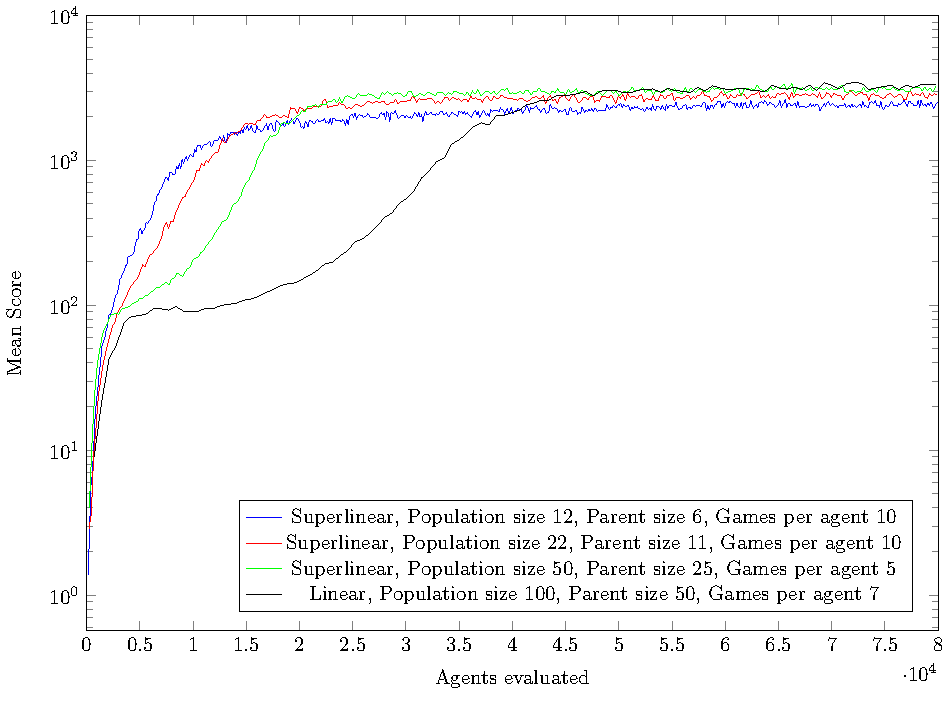
\includegraphics[scale=0.8]{data/cma_population_offspring/bestofall_population/PlotFile.pdf}
\caption{Best performing configurations of all population sizes \label{CMABestConfigPlot}}
\end{figure}

From table \ref{CMABestConfigTable} and figure \ref{CMABestConfigPlot}, we can see that
Linear recombination type, with population size 100, parent size 50 and 7 games per agent
(black) yields a better score compared to Superlinear with population size 50, parent size 25 and 5 games per agent (green).
However, green has a much faster convergence than black and almost reaches the same score.\\

\textbf{Analysis and discussion}\\
Because the green converges almost twice as fast as black, but reaches practically the same
score, we opt to use the Superlinear with population size 50, parent size 25 and 5 games per agent for the comparison experiments.\\
Therefore, we will be using this configuration for the tuned comparison experiments.











\subsection{Comparison between the Cross Entropy and CMA-ES}

In this section, we present the actual comparison experiments between the Cross-entropy method
and CMA-ES.
In the first experiment, we conduct a comparison experiment using the 
"default" settings for both CMA-ES and the Cross-entropy method. We use this experiment to
get an initial idea of how the two algorithms compare to each other, when using the commonly
used algorithm parameters.
In the second experiment, we conduct an experiment using the "optimized" settings
specified in section \ref{optimalsettingsce} for the Cross-entropy method and section
\ref{optimalsettingscma} for CMA-ES.\\
These experiments are used to conclude whether CMA-ES or the Cross-entropy method
is the better algorithm for learning Tetris.


\subsubsection{Initial comparison}
For the initial comparison we use the Bertsekas featureset, since the same featureset
was used for verifying the Cross Entropy implementation. Furthermore, others researchers
has used the Bertsekas featureset as a benchmarking standpoint \citep{thiery:09} \&
\citep{szita:06}.\\
The goal of this comparison is to get an initial idea of how the Shark implementation of
CMA compares to Cross Entropy.\\

\textbf{Results}

Using Cross Entropy with the constant noise setting and CMA with an initial step-size
of $0.5$, we get the following results, seen in figure \ref{fig:CMA_VS_CE_00}.\\

\begin{figure}[H]
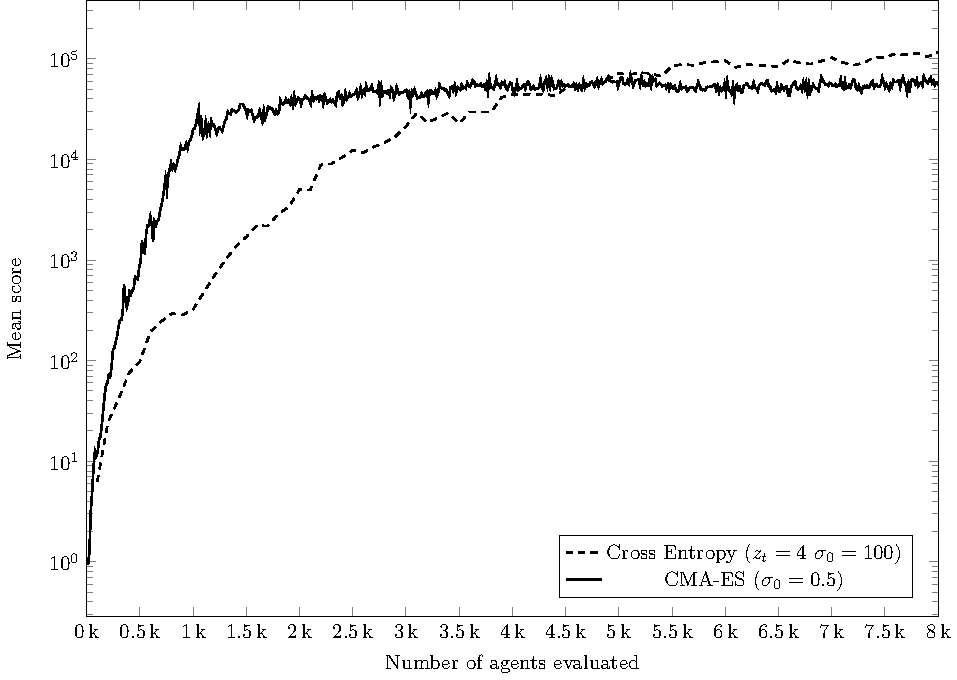
\includegraphics[scale=1]{plots/cmaCePlot}
\caption{Initial comparison between CMA-ES and Cross Entropy \label{fig:CMA_VS_CE_00}}
\end{figure}

As figure \ref{fig:CMA_VS_CE_00} reveals that CMA converges faster,
but reaches a local optimum at around 2,000 games played. Meanwhile CE has a 
slower convergence but reaches a better mean score compared to CM at around 5,500
agents evaluated. In detail, CMA on average reaches a score of 50,000 rows, and
CE reaches a score of 100,000.\\

\comment{Add the raw graphs to appendix}

\textbf{Analysis and discussion}

These results clearly defy our initial hypothesis as we predicted
for CMA to outperform CE, due to its more sophisticated nature. 
One reason for this outcome could possibly be that
CMA has a very little population size compared to Cross Entropy,
which could be a decisive lack as the objective function is noisy with 
a high variance. These results indicate a need to adjust the CMA
configuration, to prevent the too fast convergance.

Among the possible adjustments are:\\
\\
\textit{Enlargment of population size}\\
As the population size is quite small (only around 13)
for this experiment, the CMA algorithm might not be able
extract enough information at each generation. As seen in 
section \ref{optimalsettingsce}, CE looses performance as 
thepopulation size is set too low. This might be a problem 
that counts for CMA as well. In figure \ref{fig:CMA_VS_CE_00},
the CMA algorithm has much the same shape as \\
\\
\textit{Evaluate each agent multiple times}\\
A posible source of poor performance could be 
that the ranking of agents becomes very difficult
due to high noise. To better verify the actual
performance of an agent, it could be evaluated 
multiple times and let the mean of the evaluations
determine it's ranking.\\
\\
\textit{Change the recombination type}\\
As described in section \ref{CMAtheory}, 
the CMA algorithm is not bound to update its 
new mean to just the centroid of the selected 
vectors. Instead, it can weight better solutions
more heavily when moving its mean. When doing so,
it risks biasing vectors that appear to be better 
but in reality, just by faulty ranking, should
not be considered a good agent.\\
\\
None of the experiments seen so far has allowed a 
consistent mean score of more 
than 200,000. This brings concern into 
consideration, that it might be the objective function
that poses a natural limit on the score.
In this case the objective function
models playing Tetris with the Bertsekas featureset. 
It is unkown to us
whether it's possible to construct an agent 
with a mean score of more than
200,000 lines on average. 
Yet, as our aim is not to find the best controller,
untill both algorithms reaches the same upper limit 
of scores theres is no need
to alter the featureset just to
expand the maximum score reachable.\\
\\
Yet, to minimize the likelihood 
that the featureset were the cause of the 
poor performance of CMA, it seemed 
appropiate to conduct a similar comparison 
using another featureset. 
To speed up the process, the game difficulty were 
adujsted to casue agents to fail faster.
The increased difficulty and alternate
featureset is described in 
further detail in section \ref{compoffeatureset}.



\subsubsection{Tuned comparison \label{tunedComparison}}






